\documentclass[10pt]{article}
\usepackage[a4paper,landscape,margin=0.72in]{geometry}
\usepackage[T1]{fontenc}
\usepackage{lmodern,amsmath,amssymb,graphicx,hyperref}
\title{A checked point in the actual weighted-Proj chart overlap}
\author{Formal proof packet}
\date{28 October 2026}
\begin{document}
\maketitle
\noindent For every field $K$ and coefficient tuple, the new Lean theorem constructs a point of the actual weighted-$\operatorname{Proj}$ curve belonging to both its $X$- and $Z$-basic opens. No separability hypothesis is needed for this point-level statement. Pinned Lean 4.34.1 exited zero; the direct axiom audit lists only \texttt{propext}, \texttt{Classical.choice}, and \texttt{Quot.sound}.

\section*{Witness and checked dependencies}
The infinity-chart coordinate ring is a domain, so its zero prime exists. The previously checked $\bar z\ne0$ lemma places that prime in $D(\bar z)$. The existing checked cross-chart theorem identifies $D(\bar z)$ with the inverse image of the actual weighted-$\operatorname{Proj}$ $Z$-open under the $X$-chart map. By definition, this map lands in the $X$-open. The source theorem combines these facts into an explicit point of the intersection.

\section*{Remaining boundary}
The new theorem proves nonempty overlap only. A whole-curve \texttt{IsIntegral} instance still needs the two chart-domain properties transported across their scheme isomorphisms, then irreducibility and reducedness glued over the checked two-open cover. The affine chart domain currently requires a separable quintic. Principal divisors at all closed points, Picard-class transport, and compiled runtime semantics remain open. The Markdown and CSV give exact declarations and statuses. No DLP experiments or cost comparisons were run.

\clearpage
\section*{Proof dependencies}
\begin{center}
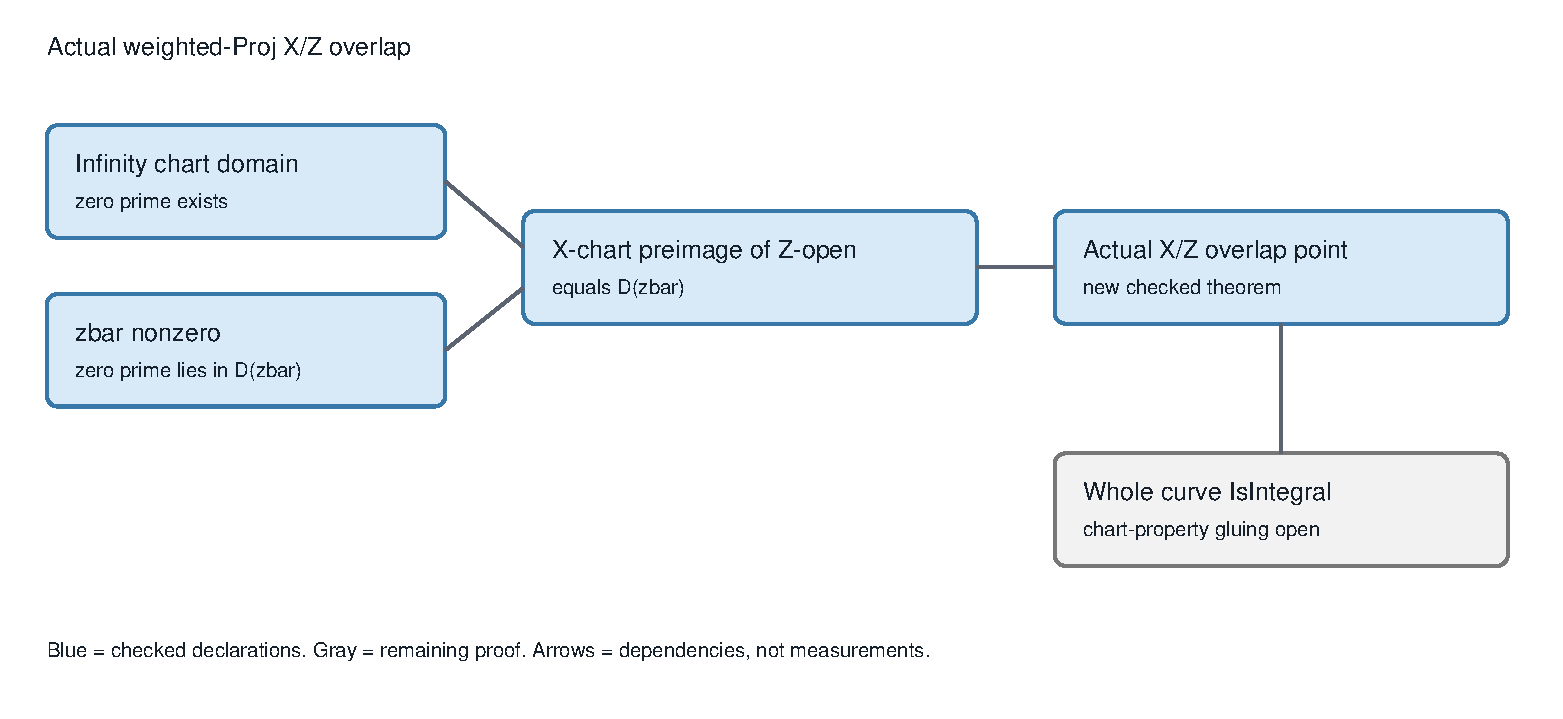
\includegraphics[width=0.96\textwidth,height=0.78\textheight,keepaspectratio]{projective-overlap-nonempty-figure.pdf}
\end{center}
\noindent Blue nodes are checked; the gray node is a remaining proof obligation. Arrows are dependencies, not performance measurements.
\end{document}
